\section{Results}
\label{sec:results}

\subsubsection{Tuning Learning Rate and Minibatch Size}
\subsubsubsection*{Logistic Regression}
% Eksempel for figurer
\begin{figure}[htbp]
	\centering
	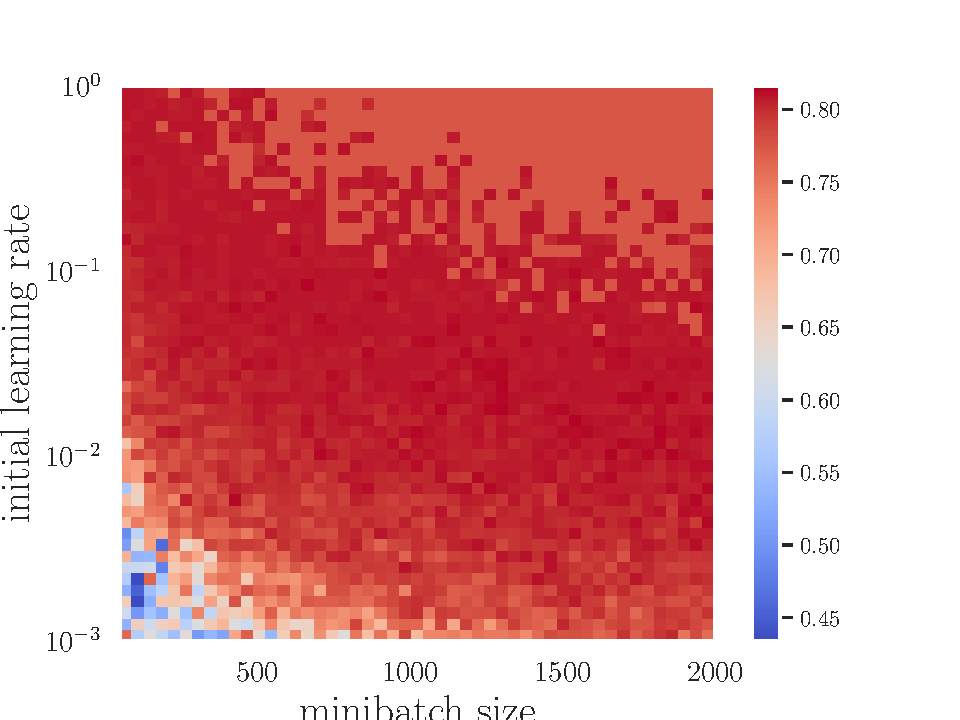
\includegraphics[width=0.5\textwidth]{LogRegTune}
	\caption{Heatmap showing the accuracy of the Logistic Regression for different
    values of the minibatch sizes and initial learning rates.}
	\label{fig:TuneLogReg}
\end{figure}


\subsubsection*{Optimal Parameters and Associated Results}

\subsubsection{Verification by Comparison to Scikit-Learn}

\subsubsection{Neural Networks for Regression on Franke's Function}


% Eksempel for figurer
\begin{table}[htbp]
<<<<<<< HEAD
\caption{Fraction of true and false negatives and positives for Neural network (NN), Logistic regression (LR) and SciKitLearn's neural network (SKL)}
	\begin{tabular}{l  l  r  r  r} 
		 & & \textbf{LR} & \textbf{NN} & \textbf{SKL} \\
=======
\caption{Percentage of true and false negatives and positives for Neural network (NN), Logistic regression (LR) and SciKitLearn's neural network (SKL)}
	\begin{tabular}{l  l  r  r  r}
		 & & \textbf{NN} & \textbf{LR} & \textbf{SKL} \\
>>>>>>> be25d18310e12616b3c7f4730f931e2f487e1f2b
		 \hline
		Positive & True & & & \\
		%\cline{2-5}
<<<<<<< HEAD
		 & False &  & & \\ 
		 \hline
		Negative & True & &  & \\ 
=======
		 & False & & & \\
		 \hline
		Negative & True & & & \\
>>>>>>> be25d18310e12616b3c7f4730f931e2f487e1f2b
		%\cline{2-5}
		& False & & & \\
	\end{tabular}
\label{tab:confusion}
\end{table}

\begin{figure}[htbp]
	\centering
	%\includegraphics[width=0.5\textwidth]{}
	\caption{}
	\label{fig:}
\end{figure}
